\section{Vollständige und rohe Ergebnisse der Nutzerbefragung}

\begin{table}[H]
    \centering
    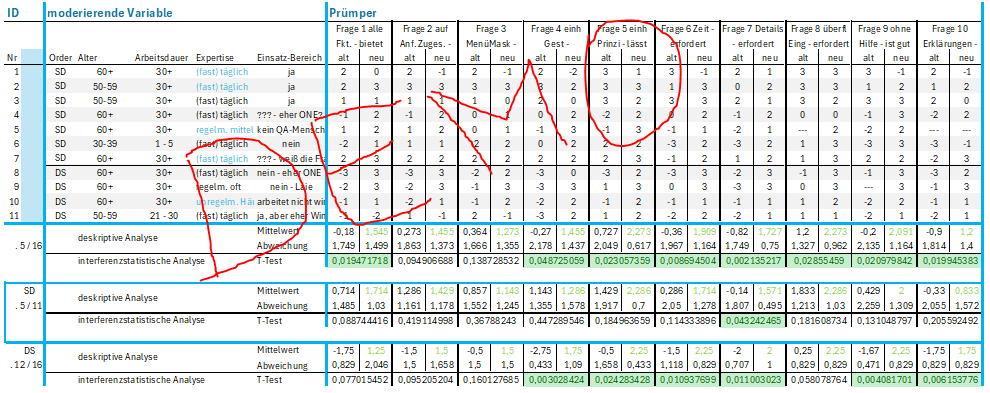
\includegraphics[width=0.65\textheight, angle=90]{Anhänge/Nutzerbefragung/prümper-Tabelle_demo.PNG}
    \caption{Nutzerbefragung nach Prümper - Tabellarische Daten}
    \label{tab:Nutzerbefragung:rohe_Daten}
\end{table}

% Boxplots
\begin{figure}[H]
    \centering
    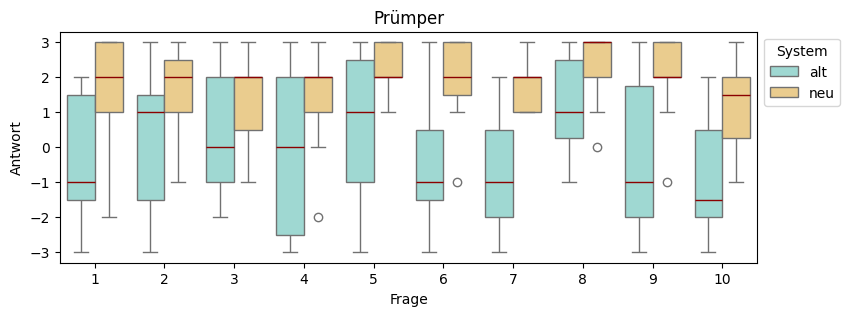
\includegraphics[width=1\linewidth]{Diagramme/pruemper_all.png}
    \caption{Auswertung der Nutzerbefragung (Daten aus \autoref{tab:Nutzerbefragung:rohe_Daten})\textcolor{red}{Titel ändern! y-Achsenbeschriftungen - gut(3) schlecht(-3)!}}
    \label{fig:pruemper_all}
\end{figure}

% Tabelle
\begin{table}[H]
%\centering
\justifying
\begin{tabular}{|l|c|c|c|}
\hline
Frage 1   & $\Bar{x}$ & $\Tilde{x}$ & $\sigma$ \\ \hline
alt       & -0,2      & -1          & 1,75     \\ \hline
neu       & 1,55      & 2           & 1,5      \\ \hline
%Differenz & +1,75     & +3          & -        \\ \hline
%\end{tabular}
%\begin{tabular}{|l|c|c|c|}
\hline
Frage 2   & $\Bar{x}$ & $\Tilde{x}$ & $\sigma$ \\ \hline
alt       & xxxx      &  xx         &  xxxx    \\ \hline
neu       & xxxx      &  xx         &  xxxx    \\ \hline
%Differenz &           &             & -        \\ \hline
%\end{tabular}
%\begin{tabular}{|l|c|c|c|}
\hline
Frage 3   & $\Bar{x}$ & $\Tilde{x}$ & $\sigma$ \\ \hline
alt       & xxxx      &  xx         &  xxxx    \\ \hline
neu       & xxxx      &  xx         &  xxxx    \\ \hline
%Differenz &           &             & -        \\ \hline
%\end{tabular}
%\begin{tabular}{|l|c|c|c|}
\hline
Frage 4   & $\Bar{x}$ & $\Tilde{x}$ & $\sigma$ \\ \hline
alt       & xxxx      &  xx         &  xxxx    \\ \hline
neu       & xxxx      &  xx         &  xxxx    \\ \hline
%Differenz &           &             & -        \\ \hline
%\end{tabular}
%\begin{tabular}{|l|c|c|c|}
\hline
Frage 5   & $\Bar{x}$ & $\Tilde{x}$ & $\sigma$ \\ \hline
alt       & xxxx      &  xx         &  xxxx    \\ \hline
neu       & xxxx      &  xx         &  xxxx    \\ \hline
%Differenz &           &             & -        \\ \hline
\end{tabular}
\begin{tabular}{|l|c|c|c|}
\hline
Frage 6   & $\Bar{x}$ & $\Tilde{x}$ & $\sigma$ \\ \hline
alt       & xxxx      &  xx         &  xxxx    \\ \hline
neu       & xxxx      &  xx         &  xxxx    \\ \hline
%Differenz &           &             & -        \\ \hline
%\end{tabular}
%\begin{tabular}{|l|c|c|c|}
\hline
Frage 7   & $\Bar{x}$ & $\Tilde{x}$ & $\sigma$ \\ \hline
alt       & xxxx      &  xx         &  xxxx    \\ \hline
neu       & xxxx      &  xx         &  xxxx    \\ \hline
%Differenz &           &             & -        \\ \hline
%\end{tabular}
%\begin{tabular}{|l|c|c|c|}
\hline
Frage 8   & $\Bar{x}$ & $\Tilde{x}$ & $\sigma$ \\ \hline
alt       & xxxx      &  xx         &  xxxx    \\ \hline
neu       & xxxx      &  xx         &  xxxx    \\ \hline
%Differenz &           &             & -        \\ \hline
%\end{tabular}
%\begin{tabular}{|l|c|c|c|}
\hline
Frage 9   & $\Bar{x}$ & $\Tilde{x}$ & $\sigma$ \\ \hline
alt       & xxxx      &  xx         &  xxxx    \\ \hline
neu       & xxxx      &  xx         &  xxxx    \\ \hline
%Differenz &           &             & -        \\ \hline
%\end{tabular}
%\begin{tabular}{|l|c|c|c|}
\hline
Frage 10   & $\Bar{x}$ & $\Tilde{x}$ & $\sigma$ \\ \hline
alt       & xxxx      &  xx         &  xxxx    \\ \hline
neu       & xxxx      &  xx         &  xxxx    \\ \hline
%Differenz &           &             & -        \\ \hline
\end{tabular}

\begin{tabular}{ll}
\multicolumn{2}{l}{verwendete Formelzeichen:} \\ \hline
$\Bar{x}$          & Mittelwert               \\
$\Tilde{x}$        & Median                   \\
$\sigma$           & Standardabweichung      
\end{tabular}
\caption{Zusammenfassung der Ergebnisse der Nutzerumfrage (Weiterverarbeitung der Daten aus \autoref{tab:Nutzerbefragung:rohe_Daten}) \textcolor{red}{TODO: fehlende Werte}}
\label{tab:Nutzerbefragung:mittelwerte}
\end{table}